\section{Segmentation}

Current \espina\ version offers one semi-automatic tool to create new
segmentations, the Seed Grow Segmentation Tool. In addition, new segmentations
an be created using drawing tools exposed in the next section.

\subsection{Seed Grow Segmentation}

This tool provides a semi-automated segmentation algorithm. Select a voxel
belonging to the object being segmented. A new segmentation will be createad
including all voxel which are equivalent (in gray scale values) to the selected
one, the seed.\\
If you have defined your own ``volume of interest'', then that is used instead of
the default one when applying the algorithm. The volume of interest will limit the
effect of the algorithm to the space enclosed within the volume.\\

\begin{figure}[H]
\centering
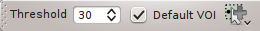
\includegraphics{fig/SeedGrowSegmentation}
\caption{Seed grow toolbar.}
\end{figure}
\vspace{0.3cm}

\begin{tabular}{| m{1.3cm} | m{12cm} |}
\hline
\textbf{Button} & \textbf{Description}\\
\hline
& %No icon
\textbf{Threshold}: Gray scale difference admisible to consider a voxel equal to
the one selected as seed. \\
\hline
& %No icon
\textbf{Default VOI}: Determine whether or not a rectangular volume of interest
centered on the selection point is applied. The size of the default VOI can be
specified in the Seed Grow Segmentation Settings Panel.\\
\hline

\includegraphics[width=0.6cm]{../../frontend/toolbar/seedgrow/rsc/pixelSelector} &
\textbf{Pixel Selector}: Create a new segmentation using the voxel under the
cursor as seed for the Seed Grow Algorithm.\\
\hline

\includegraphics[width=0.6cm]{../../frontend/toolbar/seedgrow/rsc/bestPixelSelector} &
\textbf{Best Pixel Selector}: Create a new segmentation placing the seed in the
voxel whose gray scale value is the closest to the one specified in the Seed
Grow Segmentation Settings Panel (black by default). Best pixel selector check
all voxels within the area under the cursor's region.\\
\hline
\end{tabular}

\vspace{0.3cm}
\begin{bclogo}[couleur = yellow!33, logo= \bcbook]
{Tip} Use Ctrl+Wheel to change threshold while this tool is active.
\end{bclogo}
\vspace{0.3cm}

Best voxel is defined in terms of gray scale similarity with a
reference gray scale value. The reference value can be configured at Seed Grow
Segmentation settings panel.\\

\subsection{Seed Grow previsualization}

Before applying the tool the user can use a partial preview that will show what
voxels will be initially selected with the chosen algorithm. The preview will 
respect the limitations imposed by the ``volume of interest'' is the user has
defined one. \\

The preview is activated using the \textbf{shift} key, and while the shift key is
holded down a preview of the growing algorithm will be shown under the mouse cursor.\\

\begin{bclogo}[couleur = yellow!33, logo=\bcattention]
{Note} The preview is only partial since it only shows what voxels will be selected
initially in in the current slice and doesn't take into account the underlying connectivity.
Therefore it is possible that the result of applying the tool differs from what was shown
in the preview. This is done this way for performance reasons.
\end{bclogo}\\


